\documentclass[tikz]{standalone}
\usepackage{amsmath}
\usepackage{amsfonts}

\begin{document}

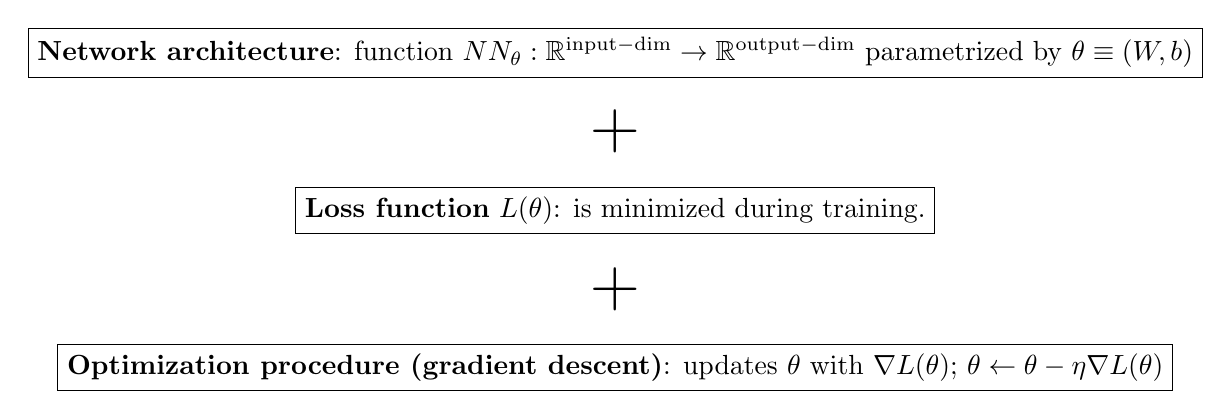
\begin{tikzpicture}
    \node[rectangle,draw] (i1) at (0,0) {\textbf{Network architecture}: function $NN_\theta:\mathbb{R}^\mathrm{input-dim}\to\mathbb{R}^\mathrm{output-dim}$ parametrized by $\theta \equiv (W,b)$ };
    \node[below of=i1] (p1) {\Huge+};
    \node[rectangle,draw, below of=p1] (i2) {\textbf{Loss function} $L(\theta)$: is minimized during training.};% $\implies$ \textbf{reconstruction error} $||M - \mathcal{R}\circ\mathcal{P}(M)||$};
    \node[below of=i2] (p2) {\Huge+};
    \node[rectangle,draw, below of=p2] (i3) {\textbf{Optimization procedure (gradient descent)}: updates $\theta$ with $\nabla{}L(\theta)$; $\theta \leftarrow \theta - \eta\nabla{}L(\theta)$};
\end{tikzpicture}

\end{document}